\documentclass[]{article}

 \title{PX3350 - Project Diary \linebreak
 \textbf{Hofstadter’s butterfly in optical ring-resonator array}\vspace{-2em}}
 \date{\parbox{\linewidth}{\centering%
   \today\endgraf\smallskip
   Author: FULL NAME (STUDENT NUMBER) \endgraf \smallskip
   Project Supervisor: SUPERVISOR NAME\endgraf\medskip \vspace{2.5cm}
   
\includegraphics[width=7cm]{coat-of-arms.jpg} \endgraf\medskip
   Cardiff University \endgraf\medskip
   School of Physics and Astronomy \endgraf\medskip
   }}

 \usepackage{pgfplots}
 \usepackage{multicol}
 \usepackage{amsmath, amsfonts, amssymb, amsthm}
 \usepackage[margin=1in]{geometry}
 \usepackage{physics}
 \usepackage{todonotes}
 \usepackage{fancybox}
 \usepackage{tikz}
 \usepackage{pgfplotstable}
 \usepackage{listings}
 \usepackage{float}
 \usepackage{circuitikz}
 \usepackage{comment}
 \usepackage{longtable}
 \usepackage{pst-magneticfield}
 \usepackage{graphicx}
 \usepackage{esint}
 \usepackage[nottoc,numbib]{tocbibind}


 \usepackage[utf8]{inputenc}
 \usepackage{dirtytalk}

 \pgfplotsset{compat=1.7}
 \graphicspath{ {./Images/} }
 \setlength{\columnsep}{0.75cm}

 \usetikzlibrary{arrows.meta,quotes,angles,calc,patterns,decorations.pathmorphing,decorations.markings, positioning}
 \usepgfplotslibrary{fillbetween}
\begin{document}

\maketitle
  \pagebreak
  \tableofcontents
  \listoffigures
  \pagebreak


% Used to keep note of any questions asked about the project to supervisor  
\section{Questions}

    \begin{multicols*}{2}
        
        \subsection{**QUESTION**}

            **ANSWER TO QUESTION**



    \end{multicols*}

%Place to store definitions of all terms, formulas, or phenomena encountered that I didn't know previously     
\section{Definitions}

    \begin{multicols*}{2}

        \subsection{**TERM NAME**}


            **NOTES ON THE GIVEN TERM**
            
            %When directly copying from external source it can be done this way to ensure you know down the line this isn't an original statement. 
            \begin{quote}
                "**QUOTE FROM EXTERNAL SOURCE**" \\ 
                %Part below can either include the name of the person or a BiBTeX reference which will be automatically categorized
                \hspace*{\fill} (**SOURCE OF QUOTE**)
            \end{quote}
            
            %If any pictures or graphs are included they can be added this way to ensure they are properly referenced and can be cited in later sections
            \begin{figure}[H]
                \begin{center}
                    %Diagrams, Puctures, Graphs, etc. are added this way
                    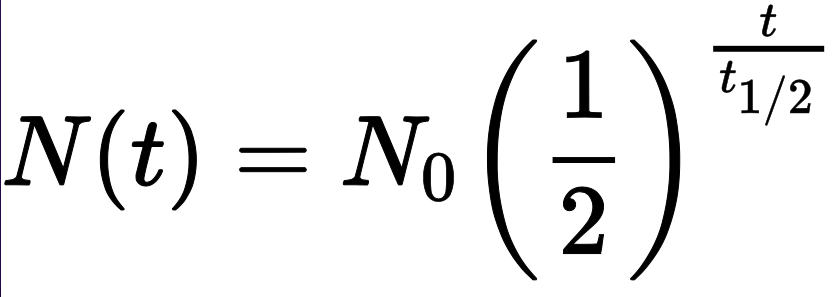
\includegraphics[width=\linewidth]{Diagrams/photoOfFormula.png}
                \end{center}
                %Adds a discription to the figure
                \caption{\textit{Equation blah blah blah with $k=30$ math bit referencing its source \cite{hofstadter1976energy}}}
                %Label allows the figure to be dynamically referenced in other places
                \label{fig:hofButterfly}
            \end{figure}

        \subsection{**NEXT TERM**}
        

    \end{multicols*}


        
%Any readings of papers or watching lectures done is kept here
\section{Reading}

    \begin{multicols*}{2}
        
    %Paper title with BiBTeX reference that can be later easily copied to Report
    \subsection{**PAPER TITLE* \cite{hofstadter1976energy}}

    
    \subsection{**LECTURE TITLE** \cite{kim_2014}}

        **NOTES**

        \begin{quote}
            **QUOTE FROM LECTURE**
        \end{quote}


    \end{multicols*}


    %Place to keep notes on any experiments done, how they were preformed, etc. 
    \section{Experimental}

        %Dated sections about each instance of working in lab or on experiments whether in lab environment or simulations
        \subsection{**DATE**}

            %Short description of the experiment or simulation to quickly see what was done that day. 
            \textit{**BRIEF DESCRIPTION OF WHAT WAS DONE**}

            **ANY NOTES PER DISCRETION**

    %Working out for any equations, etc. Do not include numerical calculations, but can contain small sample of results from working shown.
    \section{Calculations}

        \subsection{**NAME OF WORKING**}

            Blah blah we are using blah blah and blah blah to derive blah blah

            %Entry of single equation
            \begin{equation}
                f(x)=h_1 e^{-\frac{(x-\mu_1)^2}{2\sigma_1^2}}+h_2 e^{-\frac{(x-\mu_2)^2}{2\sigma_2^2}}+c
                %Label to allow easier referencing of equation later in text
                \label{eq:dubGauss}
            \end{equation}


            %Entry for working out with labels that can be used to reference parts later
            \begin{align}
                E_1&=A+B \label{eq:1}\\
                 \begin{split}
                  E_2&=(C-D)E_1 \label{eq:2}\\
                  &\quad +[(1-R)+R(1-Y)\\
                  &\quad +\pi(1-\delta)]E_2\\
                  &\quad +F\cdot E_3
                 \end{split}\\
                E_3 &=(\pi\cdot \chi)-(R\cdot E_1)-(RY\delta\cdot E_2) \label{eq:3}
            \end{align}


        
    \begin{multicols}{2}

        
    \end{multicols}



    \begin{equation}
        N=\frac{f}{d}
        \label{eq:fstop}
    \end{equation}

  
    

%References section

  \nocite{*}
  \bibliography{References}
  \bibliographystyle{abbrv}


\end{document}
